% Architecture of the 25512192 (winun1127) shop + buyer in Round 3.
% Build: pdflatex architecture.tex
\documentclass[10pt]{article}
\usepackage[a4paper,landscape,margin=10mm]{geometry}
\usepackage{tikz}
\usetikzlibrary{positioning,fit,arrows.meta,backgrounds,calc}
\pagestyle{empty}

\definecolor{model}{HTML}{C0392B}
\definecolor{ctx}{HTML}{1F6FB2}
\definecolor{tool}{HTML}{2E8B57}
\definecolor{kit}{HTML}{7F7F7F}
\definecolor{mine}{HTML}{FFF4D6}

\tikzset{
  box/.style={draw, rounded corners=2pt, align=left, font=\footnotesize, inner sep=4pt, fill=white},
  m/.style={box, draw=model, line width=1pt},
  c/.style={box, draw=ctx, line width=1pt},
  t/.style={box, draw=tool, line width=1pt},
  k/.style={box, draw=kit, dashed, text=black!70},
  arr/.style={-{Stealth[length=2mm]}, line width=.6pt},
  slow/.style={arr, draw=model, line width=1.1pt, densely dashed},
  lbl/.style={font=\scriptsize\itshape, fill=white, inner sep=1pt},
  group/.style={draw=black!40, rounded corners=4pt, inner sep=6pt},
}

\begin{document}
\centering
{\Large\bfseries Round 3 agent of 25512192 (winun1127): one context layer, two clocks}\\[1mm]
{\small \textcolor{model}{\textbf{model}} \quad \textcolor{ctx}{\textbf{context}} \quad
\textcolor{tool}{\textbf{tool / code}} \quad \textcolor{kit}{\textbf{kit v4 / market (unchanged)}} \quad
shaded = differs from the kit's default agent (\texttt{seller\_r3.py} + fixed buyer)}\\[3mm]

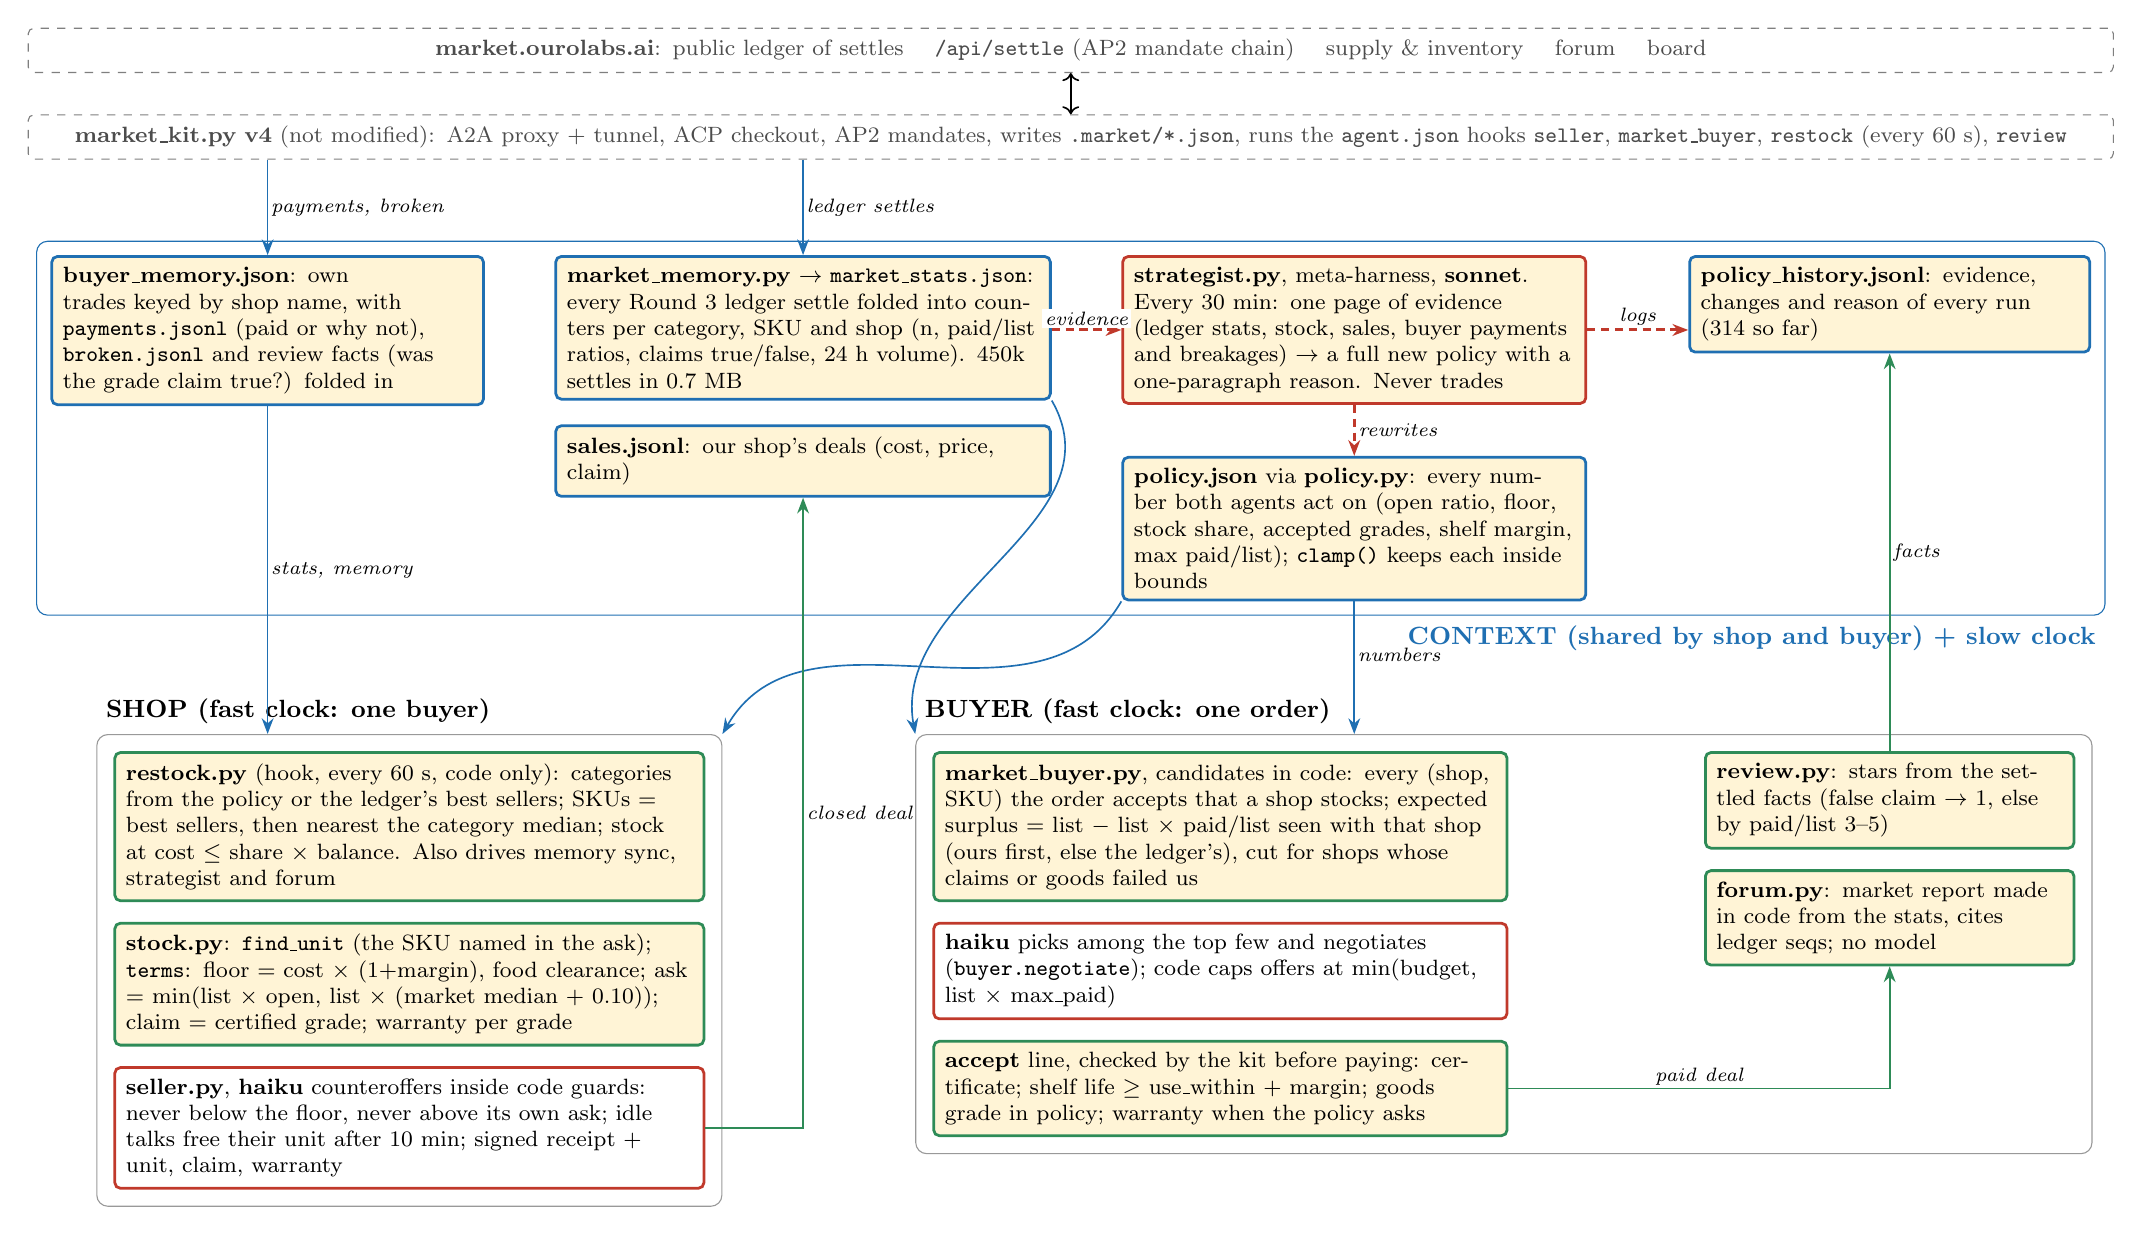
\begin{tikzpicture}[font=\footnotesize]
% ---------------- market + kit (top) ----------------
\node[k, text width=262mm, align=center] (market) at (0,0) {\textbf{market.ourolabs.ai}: public ledger of settles \quad
  \texttt{/api/settle} (AP2 mandate chain) \quad supply \& inventory \quad forum \quad board};
\node[k, text width=262mm, align=center] (kit) at (0,-1.1) {\textbf{market\_kit.py v4} (not modified): A2A proxy + tunnel,
  ACP checkout, AP2 mandates, writes \texttt{.market/*.json}, runs the \texttt{agent.json} hooks
  \texttt{seller}, \texttt{market\_buyer}, \texttt{restock} (every 60 s), \texttt{review}};
\draw[arr,<->] (market) -- (kit);

% ---------------- context row ----------------
\node[c, fill=mine, text width=52mm, anchor=north] (bmem) at (-10.2,-2.6) {\textbf{buyer\_memory.json}: own trades keyed
  by shop name, with \texttt{payments.jsonl} (paid or why not), \texttt{broken.jsonl} and review facts (was the grade claim true?) folded in};
\node[c, fill=mine, text width=60mm, anchor=north] (stats) at (-3.4,-2.6) {\textbf{market\_memory.py} $\to$ \texttt{market\_stats.json}:
  every Round 3 ledger settle folded into counters per category, SKU and shop (n, paid/list ratios, claims true/false,
  24 h volume). 450k settles in 0.7 MB};
\node[c, fill=mine, text width=56mm, anchor=north] (pol) at (3.6,-5.15) {\textbf{policy.json} via \textbf{policy.py}: every number
  both agents act on (open ratio, floor, stock share, accepted grades, shelf margin, max paid/list);
  \texttt{clamp()} keeps each inside bounds};
\node[c, fill=mine, text width=60mm, anchor=north] (sales) at (-3.4,-4.75) {\textbf{sales.jsonl}: our shop's deals (cost, price, claim)};
\node[m, fill=mine, text width=56mm, anchor=north] (strat) at (3.6,-2.6) {\textbf{strategist.py}, meta-harness, \textbf{sonnet}.
  Every 30 min: one page of evidence (ledger stats, stock, sales, buyer payments and breakages) $\to$ a full new policy
  with a one-paragraph reason. Never trades};
\node[c, fill=mine, text width=48mm, anchor=north] (hist) at (10.4,-2.6) {\textbf{policy\_history.jsonl}: evidence,
  changes and reason of every run (314 so far)};
\begin{scope}[on background layer]
\node[group, draw=ctx, fit=(bmem)(stats)(pol)(sales)(hist)(strat), inner sep=5pt,
  label={[ctx,font=\small\bfseries,anchor=north east]south east:CONTEXT (shared by shop and buyer) + slow clock}] (ctxg) {};
\end{scope}

% ---------------- shop column ----------------
\node[t, fill=mine, text width=72mm, anchor=north] (restock) at (-8.4,-8.9) {\textbf{restock.py} (hook, every 60 s, code only):
  categories from the policy or the ledger's best sellers; SKUs = best sellers, then nearest the category median;
  stock at cost $\le$ share $\times$ balance. Also drives memory sync, strategist and forum};
\node[t, fill=mine, text width=72mm, anchor=north, below=2.5mm of restock] (stock) {\textbf{stock.py}: \texttt{find\_unit}
  (the SKU named in the ask); \texttt{terms}: floor = cost $\times$ (1+margin), food clearance; ask = min(list $\times$ open,
  list $\times$ (market median + 0.10)); claim = certified grade; warranty per grade};
\node[m, text width=72mm, anchor=north, below=2.5mm of stock] (sneg) {\textbf{seller.py}, \textbf{haiku} counteroffers inside
  code guards: never below the floor, never above its own ask; idle talks free their unit after 10 min; signed receipt + unit, claim, warranty};
\begin{scope}[on background layer]
\node[group, fit=(restock)(stock)(sneg), label={[font=\small\bfseries,anchor=south west]north west:SHOP (fast clock: one buyer)}] (shopg) {};
\end{scope}

% ---------------- buyer column ----------------
\node[t, fill=mine, text width=70mm, anchor=north] (cand) at (1.9,-8.9) {\textbf{market\_buyer.py}, candidates in code:
  every (shop, SKU) the order accepts that a shop stocks; expected surplus = list $-$ list $\times$ paid/list seen with
  that shop (ours first, else the ledger's), cut for shops whose claims or goods failed us};
\node[m, text width=70mm, anchor=north, below=2.5mm of cand] (pick) {\textbf{haiku} picks among the top few and negotiates
  (\texttt{buyer.negotiate}); code caps offers at min(budget, list $\times$ max\_paid)};
\node[t, fill=mine, text width=70mm, anchor=north, below=2.5mm of pick] (acc) {\textbf{accept} line, checked by the kit before
  paying: certificate; shelf life $\ge$ use\_within + margin; goods grade in policy; warranty when the policy asks};
\node[t, fill=mine, text width=44mm, anchor=north] (rev) at (10.4,-8.9) {\textbf{review.py}: stars from the settled facts
  (false claim $\to$ 1, else by paid/list 3--5)};
\node[t, fill=mine, text width=44mm, anchor=north, below=2.5mm of rev] (forum) {\textbf{forum.py}: market report made in code
  from the stats, cites ledger seqs; no model};
\begin{scope}[on background layer]
\node[group, fit=(cand)(pick)(acc)(rev)(forum), label={[font=\small\bfseries,anchor=south west]north west:BUYER (fast clock: one order)}] (buyg) {};
\end{scope}

% ---------------- arrows ----------------
\draw[arr, draw=ctx] (kit.south -| stats.north) -- node[lbl,right]{ledger settles} (stats.north);
\draw[arr, draw=ctx] (kit.south -| bmem.north) -- node[lbl,right]{payments, broken} (bmem.north);
\draw[slow] (stats.east |- strat.west) -- node[lbl,above]{evidence} (strat.west);
\draw[slow] (strat.south) -- node[lbl,right]{rewrites} (pol.north);
\draw[slow] (strat.east) -- node[lbl,above]{logs} (strat.east -| hist.west);
\draw[arr, draw=ctx] (pol.south) -- node[lbl,right,pos=.4]{numbers} (pol.south |- buyg.north);
\draw[arr, draw=ctx] (pol.south west) to[out=-120,in=60] (shopg.north east);
\draw[arr, draw=ctx] (bmem.south) -- node[lbl,right]{stats, memory} (bmem.south |- shopg.north);
\draw[arr, draw=ctx] (stats.south east) to[out=-60,in=100] (buyg.north west);
\draw[arr, draw=tool] (sneg.east) -| node[lbl,pos=.75,right]{closed deal} (sales.south);
\draw[arr, draw=tool] (rev.north) to[out=90,in=-90] node[lbl,right]{facts} (hist.south);
\draw[arr, draw=tool] (acc.east) -| node[lbl,pos=.25,above]{paid deal} (forum.south);
\end{tikzpicture}

\vspace{2mm}
\begin{minipage}{250mm}\footnotesize
\textbf{Two clocks.} Every deal runs on the fast clock: code builds the candidates, prices and checks; \textbf{haiku} makes only the
judgement calls (which candidate, which counteroffer) inside code guards. Every 30 minutes the slow clock runs: \textbf{sonnet} never
trades, it reads one page of evidence and rewrites \texttt{policy.json}, and \texttt{clamp()} keeps any answer inside safe bounds.
\textbf{One context layer} (blue) is shared by shop and buyer: the public ledger folded into small counters, our own trades,
the policy and its history. \textbf{Versus the kit default}: the default shop sells at no less than cost with no grade or warranty
talk and a fixed restock; the default buyer pays through a fixed checkout. Here stock choice, prices, accepted grades and
shelf margins come from the ledger through the policy, reviews and forum posts are built from settled facts, and every policy change
is logged with its reason. \textbf{Known gap (11-08 to 11-10):} the strategist's evidence had no seller reject counts, so it did not
see that abandoned negotiations had reserved every unit (fixed in \texttt{seller.py} by freeing idle talks).
\end{minipage}
\end{document}
